\documentclass[conference]{IEEEtran}
\IEEEoverridecommandlockouts
% The preceding line is only needed to identify funding in the first footnote. If that is unneeded, please comment it out.
\usepackage{cite}
\usepackage{amsmath,amssymb,amsfonts}
\usepackage{algorithmic}
\usepackage{graphicx}
\usepackage{textcomp}
\usepackage{xcolor}
\usepackage{listings}
\usepackage{pythonhighlight}
\usepackage{float}

\def\BibTeX{{\rm B\kern-.05em{\sc i\kern-.025em b}\kern-.08em
    T\kern-.1667em\lower.7ex\hbox{E}\kern-.125emX}}
\begin{document}

\hfuzz=500pt
\title{Patterns in Primes}
\author{\IEEEauthorblockN{1\textsuperscript{st} Yongyu Qiang}
\IEEEauthorblockA{\textit{Georgia Institute of Technology}}
\and
\IEEEauthorblockN{2\textsuperscript{nd} Aravinth Venkatesh Natarajan}
\IEEEauthorblockA{\textit{Georgia Institute of Technology}}
\and
\IEEEauthorblockN{3\textsuperscript{rd} Anthony Hong}
\IEEEauthorblockA{\textit{Georgia Institute of Technology}}
}

\maketitle

\begin{abstract}

\end{abstract}

\section{Introduction}
The distribution of the set of prime numbers is a topic long studied by mathematicians. We will explore some important results, with a focus on prime gaps. We will also cover Cramer's random model, a heuristic used to study distributions of seemingly random sets, such as the prime numbers. 

\section{Background}

A common result many students learn early on in number theory is about the
infinitude of prime numbers. This fact is also known as Euclid's theorem,
and we include a short summary of Euclid's original proof.

\medskip\noindent
\textbf{Euclid's Theorem.} \textit{The set of all prime numbers is larger
in cardinality than any finite collection of prime numbers.}

\smallskip\noindent
\textit{Proof.} Consider \[\{p_1, p_2, \dots, p_n\},\] some arbitrary finite
collection of
prime numbers. Let \[N = p_1p_2 \dots p_n,\] and consider $P = N + 1$. $P$ is
either prime or not prime.

First, let $P$ be prime. Then, we have constructed a new prime number and
we are done.

Now, let $P$ not be prime. Let $g$ be a prime factor of $P$. We propose that
$g \notin \{p_1, p_2, \dots, p_n\}$. To show this, suppose for contradiction that
$g \in \{p_1, p_2, \dots, p_n\}$. Then, since $p_1, p_2, \dots, p_n$ are all
factors of $N$, we have $g | N$. $g | P$ and $g | N$, so
we must also have $g | P - N$, i.e.\ $g | 1$. But $g > 1$ ($g$ is prime),
so $g$ cannot possibly divide 1. Therefore,
$g \notin \{p_1, p_2, \dots, p_n\}$, and we have found a new prime, as
required. \hfill$\square$\medskip

A natural next step from here is to explore how prime numbers
are distributed. For now, we'll focus particularly on prime
gaps and how small or large they can be. A bit of
thinking leads to the observation that there are certain
restrictions on what prime gaps can look like. First,
we can see that prime gaps can be odd only finitely many
times.

\medskip\noindent
\textbf{Proposition.} \textit{There exist only finitely many odd prime
gaps.}

\smallskip\noindent
\textit{Proof.} Notice that all primes $p > 2$ are odd. Then
$p_{n+1} - p_n$ is even for all $n > 1$, so there exists
only finitely many $n$ such that $p_{n+1} - p_n$ is odd.
\hfill$\square$\medskip

In fact, $n = 1$ yields the only odd prime gap, namely
$(p_1, p_2) = (2, 3)$ with difference 1. On the other
hand, we have a much more promising observation for large
prime gaps, namely that we can make them arbitrarily large.

\medskip\noindent
\textbf{Proposition.} \textit{There exist prime gaps of arbitrarily
large size.}

\smallskip\noindent
\textit{Proof.} We'll show that given $n \in \mathbb{Z}^+$, we
can construct an interval of size at least $n - 1$ of only
composite numbers. Then the first primes immediately before
and after this interval will have gap of at least $n$.

Let $n \in \mathbb{Z}^+$. Now consider the interval
\[[n! + 2, n! + n].\] By definition of the
factorial, we have $i|n!$ for all $i \in [2, n]$. We also
trivially have $i|i$. Therefore, we have $i|(n! + i)$, and
so $i$ is a divisor of $n! + i$ for all $i \in [2, n]$.
Then all of $[n! + 2, n! + n]$ is composite, and this
interval has size $n - 1$, as desired.
\hfill$\square$\medskip

Although this result is nice, we soon realize that it does
not give us a very strong bound, in the sense that it is
rather wasteful. To find a prime gap of
size $n$ by this method, we must consider numbers of order
$n!$. By Stirling's approximation, we have
\[n! \approx \sqrt{2\pi n} \left(\frac{n}{e}\right)^n\]
asymptotically, which is worse than exponential growth in $n$.
Put in context, our current method suggests that finding
a prime gap of size 10 requires us to find numbers
of magnitude about 3 million. In reality, we can find such a
gap of size 10 at $(p_{30}, p_{31}) = (113, 127)$, which is
much smaller than 3 million, so certainly we can
do better.

For that, we'll need better tools. Let us first define
the prime counting function $\pi(n)$.

\smallskip\noindent
\textbf{Definition.} $\pi(n) := \text{number of primes} \le n.$
\smallskip

Now we can introduce the prime number theorem,
which characterizes the growth of $\pi(n)$ as $n$ gets large.
Note that we will use this result without proof in this paper,
as even relatively simpler proofs rely on tools from
analysis.

\smallskip\noindent
\textbf{Prime Number Theorem.}
$\frac{n}{\ln(n)}$ asymptotically approximates $\pi(n)$.
Put more formally,
\[\displaystyle \lim_{n \to \infty} \frac{\pi(n)}{\frac{n}{\ln(n)}} = 1.\]
\smallskip

From this result, we can quickly argue by the pigeonhole principle
that there should exist a prime gap of size at least $\ln(n)$ in the
interval $[2, n]$. If we take buckets to be the $\frac{n}{\ln(n)}$
prime numbers less than or equal to $n$ and our pigeons to be
the integers in $[2, n]$, then by the pigeonhole principle, at least one
prime number will correspond to $\ln(n)$ or more integers, making
a gap of size at least $\ln(n)$. Note that this pigeonhole argument already gives
an asymptotically better bound for large gaps than our previous result,
albeit just barely, as we only now only need to go to $e^x$ for a gap
of size $x$ rather than $x!$.

We can also apply the same argument in reverse to get a small gap of size
at most $\ln(n)$, but getting any better bounds generally requires the
use of analysis. In an effort to avoid that, we can instead explore
the Cramer random model, which considers randomness as a method
to approximate $\pi(n)$.


\section{Cramer's Random Model}
% In this section, you should state and prove your main result,
% and provide some basic consequences and examples that help the
% reader to understand it. You may want to change this section's
% name to something more informative.
Recall that the prime number theorem tells us for
large $n$,
\[\pi(n) \approx \frac{n}{\ln(n)}.\]
But since we also have $n$ total numbers less than or equal to
$n$, we can divide by this size to get a rough prime density
$\delta(n)$:
\[\delta(n) = \frac{\pi(n)}{n} = \frac{\frac{n}{\ln{n}}}{n} = \frac{1}{\ln(n)}.\]
So for a random number $x$ in the interval $[n, n + kn]$ for
large $n$ and fixed $k$, the probability that $x$ is prime is
approximately $1 / \ln(n) \approx 1 / \ln(x)$. (As a side note, this
density $\delta(n)$ is also the rationale behind an alternate
approximation for $\pi(n)$ with the logarithmic integral
$\text{Li}(n)$ as
\[\pi(n) \approx \int_2^{n} \delta(x)\, dx = \int_2^{n} \frac{1}{\ln(x)}\, dx = \text{Li}(n),\]
which actually turns out to be a much better approximation to
$\pi(n)$ than the traditional prime number theorem. In
fact, if we assume the
Riemann hypothesis, we have that the error of $\text{Li}(n)$ from
$\pi(n)$ is bounded by $O(n^{1/2 + \epsilon})$ for any
$\epsilon > 0$, meaning that roughly the first half of the
digits of
$\text{Li}(n)$ will be correct,
but that is outside the scope of this paper.)

Equipped with this prime density, we arrive at
Cramer's random model. In 1936, Harald Cramer, a Swedish mathematician
proposed a probabilistic perspective for studying
the distribution of primes. From first inspection,
the primes don't seem to be distributed according to
any clear pattern; they seem to be rather randomly
scattered across the number line. So why don't
we treat the primes as exactly that, a random distribution?
In Cramer's original model, we assign each natural number
$x > 2$ a probability
\[p(x) = \frac{1}{\ln(x)}\]
of being prime.
The hope is that this random distribution will be within
some reasonable margin of approximating the real prime
number distribution. If we can achieve this, then not only
do we have a computationally efficient way of
estimating the prime distribution, but we can also bring
in existing tools from probability theory to help. So
let's give it a shot and see how reasonable this idea is.

We'll first explore large prime gaps and how accurate the
random model predicts them to be compared to the real
prime gaps. To do this, we computed the largest prime gap
less than or equal to a natural number $n$ for
$100 \le n \le 1.66 \times 10^5$ for both distributions.
In the random model, we assigned each natural number $x \le n$
with its probability $x/\ln(x)$ of being prime. We then sorted
these ``primes'' and calculated the largest gap between
any consecutive two elements. For the actual distribution, we
simply calculated the real largest prime gap. To mitigate the wild
varation due to the random nature of the model, we also repeated
each $x$ in the random model for a total of 100 trials and
plotted their average value.

\begin{figure}[H]
  \centering
  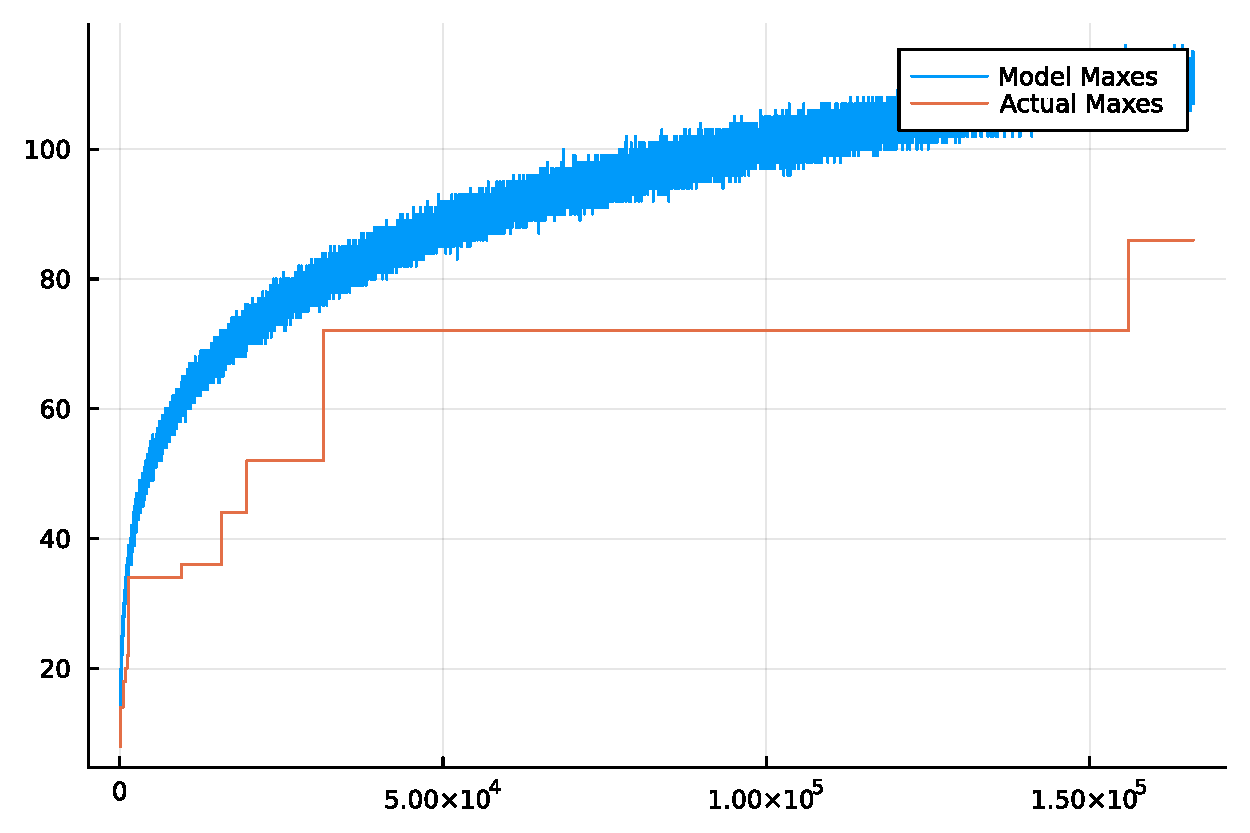
\includegraphics[width=\linewidth,keepaspectratio]{random-plot1.pdf}
  \caption{Maximum prime gaps, size of largest gap $\le n$ vs. $n$}
\end{figure}

Well\ldots that's not quite exactly what we hoped it would be,
but it's also not all that bad! We can see that for rather
small values of $x$, the two graphs line up rather nicely,
and the two graphs approach each other again around $n = 30{,}000$
(it also seems that the 100 trials did its job fairly well in reducing
random variation). The two graphs do have their differences:
the actual prime gap graph is a little too jagged for our
(relatively) continuous-looking graph to model accurately. But it
still seems that they behave similarly in a way; one could imagine that
a curve of best fit through the actual graph would look rather similar
to our model. It's not out of the world either to believe that the next
jump in the prime gap will once again approach that of
our model for larger $n$.

So not all hope is lost quite yet! We still have some more ideas.
One first observation is that in the previous iteration of the model,
we restricted our ``fake primes'' to being natural numbers. Of course,
it perhaps makes sense to do so as primes are natural numbers, but
why should we restrict ourselves in that way? What if we take $x \in \mathbb{R}$
instead of $x \in \mathbb{N}$? After all, differences, logarithms, and
division are all just as well-defined on $\mathbb{R}$, so there's theoretically
nothing preventing us from doing this.

Obviously, when we deal with $x \in \mathbb{R}$, we can
no longer assign discrete probabilities to each element,
as there's an infinite number of them! Instead, we need
to assign an actual density function like the $\delta(x)$
mentioned earlier. But $\delta(x)$ poses some problems:
for one, the integral
\[\lim_{n \to \infty} \int_2^n \delta(x)\, dx = \infty\]
doesn't converge (perhaps unsurprisingly, as there are
indeed an infinite number of primes), so we can't hope to
use it as a probability density without at least some
modifications first. But for now, we can try something
simpler.

As our first step into using a continuous model, we'll
use the simplest possible density function: the uniform
distribution. For a closed interval $[a, b]$, we can
define the following uniform density function
\[f(x) = \begin{cases}\frac{1}{b-a}, & a \le x \le b \\ 0, & \text{otherwise}.\end{cases}\]
Then, since the prime number theorem predicts roughly
$n/\ln(n)$ primes less than or equal to $n$, we can
randomly sample $n/\ln(n)$ numbers uniformly from the
interval $[2, n]$ to get an approximate distribution of
primes. So we repeat the previous experiment, with the
only change being the switch to this new method of
generating our ``fake primes.''

\begin{figure}[H]
  \centering
  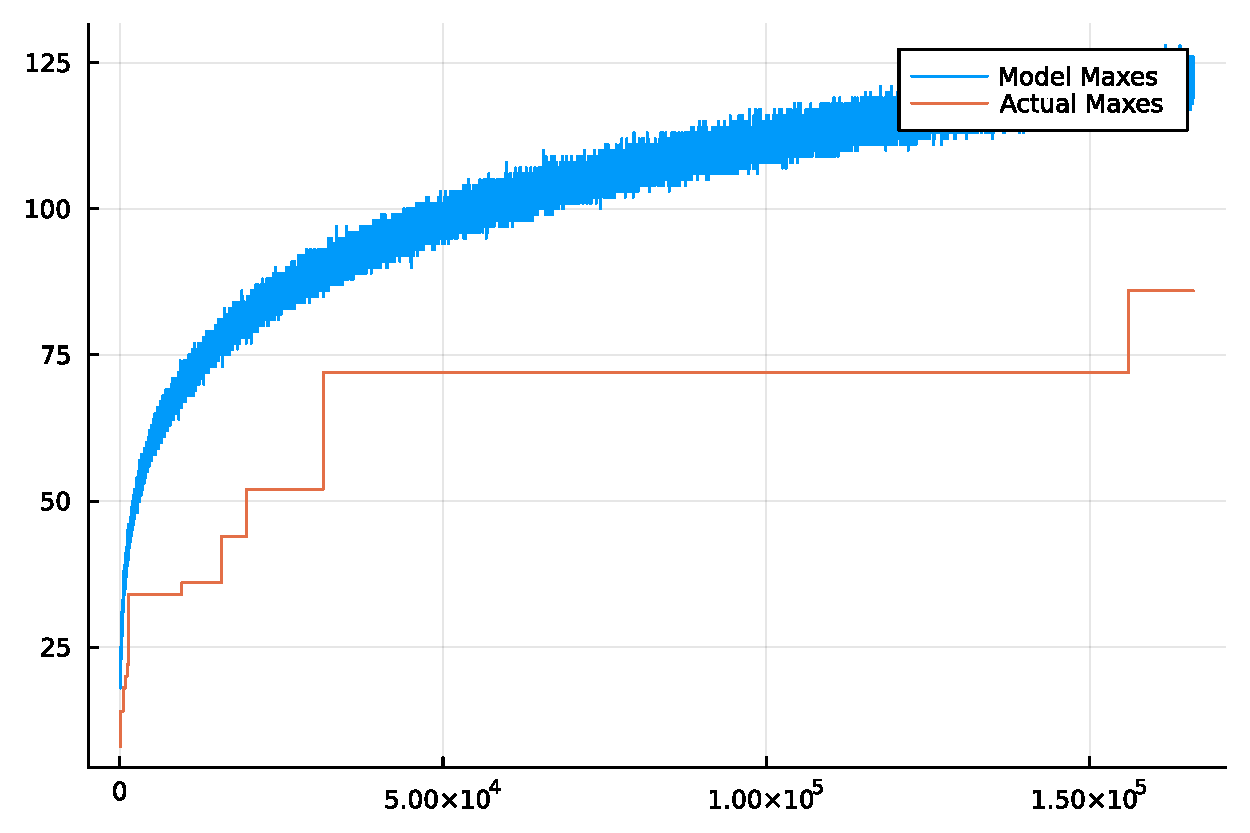
\includegraphics[width=\linewidth,keepaspectratio]{random-plot-with-reals.pdf}
  \caption{Maximum prime gaps, size of largest gap $\le n$ vs. $n$, (uniformly distributed model)}
\end{figure}

Wow, that's actually even worse than what we had before.

(note to self, explore above idea of using real numbers, and then
go into trying out other probability distributions like a Gaussian, maybe)

\vspace{2mm}
\hrule
\vspace{2mm}

\section{Improvements to Cramer's Model}

Although Cramer's original model makes a fair attempt at estimating prime number distributions, it is fundamentally flawed. The set of prime numbers is a non-random set. Primes have properties that make them deterministic. Although they exhibit pseudorandom behavior, they are not completely random. Hence, why mathematicans are obsessed with finding possible patterns. Cramer's model will generate a set of numbers that is completely random, considering only the independent probabilty $1 \ \ln(n)$. An improved version of the model would incorporate more characteristics of the actual set of prime numbers. Let's look at some of the more obvious improvements. 

% Should probably revise this section with more accurate improvements,
% http://projecteuclid.org/euclid.facm/1229619660
For any prime $p$, where $p > 2$, $p + 1$ is even and therefore cannot be prime. Currently in our model we do not consider parity, resulting in an arbitrary number of neighboring integer pairs. This never occurs in actual primes, with the exception of $(2, 3)$. Thus, let's update the probabilities of the model. To preserve the distribution in accordance to the Prime Number Theorem, lets ``move" the probability of an even number $e$ being selected, to $e + 1$. Thus, suppose $n$ is an integer greater than 2. If $n$ is even, then its updated probability of being selected is 0. If $n$ is odd, then its probability is $1 / \ln(n - 1) + 1 / \ln(n) \approx 2 / \ln(n)$.

% Maybe talk about prime triplets?
% https://math.stackexchange.com/questions/1653536/show-that-we-cannot-have-a-prime-triplet-of-the-form-p-p-2-p-4-for 

(Add models highlighting differences?)

\section{Other Applications of Cramer's Model}

The fundamental idea of Cramer's model is quite powerful. For any seemingly random set of numbers, we can emulate its density by using a random distribution. An interesting point of extension is, can we use this idea for similar sets of numbers other than the primes?

We introduce a lesser known sequence of numbers known as the Ulam numbers, named after Stanislaw Ulam, who first popularized the sequence in 1964. The Ulam sequence starts with $U_1 = 1$, $U_2 = 2$. Then for $n > 2$, $U_n$ is the smallest integer greater than $U_{n - 1}$ that can be written as a unique sum of two distinct earlier terms. The first twenty Ulam numbers are:
\[1, 2, 3, 4, 6, 8, 11, 13, 16, 18, 26, 28, 36, 38, 47, 48, 53, 57, 62, 69\]

% Psuedorandom similarity to the primes
Similar to the prime numbers, the Ulam numbers are a deterministic set. They are fixed by a clear procedure. However, it is once again a seemingly random sequence. There are no equations to describe where Ulam numbers will show up on the integer number line. Let's run a program to see the distribution of Ulam numbers across a larger sample. Finding Ulam numbers effiently is a difficult task in itself, but we can do it naively. 
% https://vixra.org/pdf/1508.0085v2.pdf

(Insert Ulam Distribution here)

% https://oeis.org/A002858

As can be seen by the distribution, Ulam numbers look quite linear. It has been shown that the first 3 million terms are close to the line $y = 13.51x$. Interestingly, Ulam himself conjectured that the natural density of Ulam numbers is 0. Meaning the distribution of Ulam numbers eventually converges to 0 as we go to infinity. But, as it turns out, calculations up to around a billion indicate that this is probably not the case. The observed density actually converges to around 0.074. 

% Revise this:
Using this density and the fact that Ulam numbers look to be quite linear, let's try to apply Cramer's model. We define a random variable such that
\[P(X = 1) = 0.074\]

(Show model vs actual Ulam numbers)

(Section on how the model trivializes analagous conjectures)
% https://chance.dartmouth.edu/chance_news/for_chance_news/Riemann/cramer.pdf
% Maybe elaborate on the importance of independence of random variables and how that trivializes conjectures
In fact, we can apply Cramer's model to any sequence with significant natural density. This tool gives us a way to confidently guess the asymptotic statistics of seemingly random sets of numbers. Proving these results rigorously is very difficult, but by random modeling, we can get the next best thing, which is a statistics backed guess. 


Cram\'er's random model uses this idea as a naive approach to emulate the distribution of prime numbers. Consider a random subset of the natural numbers, where the independent probability that a number $n$ is chosen is $1 / \ln(n)$. Let's call this random set $P'$, where $P$ is the set of actual prime numbers. Cram\'er conjectured that $P'$, which consists of our ``fake primes," accurately models the distribution of P. 

% Perhaps add summary of proof for this result
According to this heuristic, we have the resulting claim, which is known as Cram\'er's conjecture:
\[\limsup_{n \to \infty} \frac{p_{n + 1} - p_n}{(\ln p_n)^2} = 1\]
where $p_n$ denotes the $n$-th prime.

(Additional sections for these ideas (TBD)):
\begin{itemize}
  \item Problems with Cram\'er's naive model and ways we can improve it (with modern results)
  \item How Cram\'er's model fares depending on the size and location of the interval, calculating asymptomatic statistics
\end{itemize}

\section{Bertrand's Postulate}
Another problem in number theory is finding the bounds in which you would find a prime number. Of these, one of the paramount significance is \textbf{Bertrand's Postulate}: \\
Bertrand's postulate states that for an integer i $>$ 1, there is at least one prime number p
\[
    i \leq n \leq 2i 
\]
The proof for it is as follows:\\
We'll start by proving Lemma 1:
\[
    \frac{4^n}{2n} \leq \binom{2n}{n}
\]
\[
  4^n = (1 + 1)^{2n} = \sum_{k = 0}^{2n} \binom{2n}{k}
\]
Since, $\binom{2n}{0}$ is 1 and $\binom{2n}{2n}$ is 1, this is the same as
\[
    \equiv 2 + \sum_{k = 1}^{2n - 1} \binom{2n}{k} 
\]
Since the largest term in this summation is $\binom{2n}{n}$ (since for $\binom{n}{k}$, $k = n/2$ will give the largest term) and there are 2n terms, 
\[
     (2 + \sum_{k = 1}^{2n - 1} \binom{2n}{k}) \leq (2n * \binom{2n}{n})
\]
Therefore, 
\[
    \frac{4^n}{2n} \leq \binom{2n}{n}
\]
Let's now prove Lemma 2:\\
For a given prime p, let's define r as the greatest number for which $p^r | \binom{2n}{n}$. Lemma 2 is as follows, for such an r, 
\[
    p^r \le 2n
\]
Firstly, we have to introduce Legendre's Formula:\\
Legendre's Formula states that for any prime number p, and any integer n, let's define the function $v_p(n)$ as the exponent of the largest power of p that divides n. Let L = $\left\lfloor \log_{p}{n} \right\rfloor$\\
Legendre's Formula is:
\[
    v_{p}(n!) = \sum_{i = 1}^{L} {\left\lfloor \frac{n}{p^i} \right\rfloor}
\]
$\binom{2n}{n}$ can also be written as $\frac{(2n)!}{n!*n!})$\\F
Finding the largest exponent of p, r, that divides $\frac{(2n)!}{n!*n!}$ is the same as finding the largest exponent of p, r, that divides each component of $\frac{(2n)!}{n!*n!}$, i.e. $(2n)!$, $n!$

In this case, L = $\left\lfloor \log_{p}{2n} \right\rfloor$\\ Writing this in terms Legendre's Formula, we get that:
\[
    v_{p}(\binom{2n}{n}) = \sum_{i = 1}^{L} {\left\lfloor \frac{2n}{p^i} \right\rfloor} - 2\sum_{i = 1}^{L} {\left\lfloor \frac{n}{p^i} \right\rfloor}
\]
This is equivalent to:
\[
    v_{p}(\binom{2n}{n}) = \sum_{i = 1}^{L} {\left\lfloor \frac{2n}{p^i} \right\rfloor - 2\left\lfloor \frac{n}{p^i} \right\rfloor}
\]
Thinking intuitively, every term in $\sum_{i = 1}^{L} {\left\lfloor \frac{2n}{p^i} \right\rfloor - 2\left\lfloor \frac{n}{p^i} \right\rfloor}$ must either be 0 or 1.\\
If ($\frac{2n}{p^i}$ mod 1) $\geq$ 0.5 then the term would be 1, otherwise the term is 0. Therefore, the maximum value of this function would be if all the terms were equal to 1. Since we are only dealing with positive numbers, and the exponent is a monotonic function if both numbers are positive numbers,
\[
    v_{p}(\binom{2n}{n}) = r \leq L
\]
\[
    \equiv r <= \log_{p}{2n}
\]
Therefore, it follows that
\[
    p^r <= p^{\log_{p}{2n}} = 2n
\]
We are able to prove our initial Lemma 2, 
\[
    p^r <= 2n
\]
Now, we move on to proving Lemma 3:
Let's place some bounds on p for the lemma we're going to prove. If 
\[
    \frac{2n}{3} < p \leq n, then R(n, p) = 0
\]
\[
    {\binom{2n}{n}} = \frac{(2n)!}{{n!}^2}
\]
Therefore, there are 2 factors of p in the numerator, p and 2p\\
In the denominator, there are 2 factors of p, each in n!\\
The conditions mean that 3p is too large to be in the numerator\\
Due to this, the factors of p in the numerator and denominator cancel out so the greatest power of p that divides this number is 1, i.e. $p^0$, giving R = 0\\
With this, we prove Lemma 3\\
\textbf{Moving on to Lemma 4:}\\
Let's define the primorial function:
\[
    x\# = \Pi_{p \leq x} x
\]
I.e., x\# is the product of all primes less than or equal to x\\
Lemma 4 states that for x $\geq$ 3,  x\# $\leq$ $4^x$\\
We proceed by induction:\\
This claim is easily verifiable for small odd numbers. Try one yourself!\\
For even numbers, x\# = (x - 1)\# as for x $\geq$ 3, there are no even prime numbers\\
Therefore, it is also bounded by x\# $\leq$ $4^x$\\
Let's take a larger odd number, n = 2m + 1
\[
    \Pi_{p \leq n}p = \Pi_{p\leq m + 1} * \Pi_{m + 2 \leq p \leq 2m + 1}
\]
Since the Inductive Hypothesis is true for smaller odd numbers,
\[
    \Pi_{p\leq m + 1} = 4^{m + 1}
\]
Now, let's take a detour, let's look at a binomial expansion
\[
    (1 + 1)^{2m + 1} = \sum^{2m + 1}_{k = 0}{\binom{2m + 1}{k}}1^{2m + 1 - k}{1^{k}}
\]
Necessarily 
\[
    \Pi_{m + 2 \leq p \leq 2m + 1} \leq {\binom{2m + 1}{m}}
\]
Since you can notice that all the primes on the left will divide $\binom{2m+1}{m}$
\[
    \binom{2m + 1}{m} \leq \sum^{2m + 1}_{k = 0}{\binom{2m + 1}{k}}1^{2m + 1 - k}{1^{k}}
\]
\[
    \sum^{2m + 1}_{k = 0}{\binom{2m+1}{k}}1^{2m + 1 - k}{1^{k}} = 2^{2m + 1}
\]
Also, since 
\[
    {\binom{2m+1}{m}} = {\binom{2m+1}{m+1}}
\]
We can divide our bound by 2 since those numbers will be repeated\\
Therefore,
\[
    \Pi_{m + 2 \leq p \leq 2m + 1} \leq 2^{2m}
\]
Consequently,
\[
     \Pi_{p \leq n}p = 4^{m + 1} * 2^{2m}
\]
Which is equivalent to
\[
    \Pi_{p \leq n}p \leq 4^{n}
\]
Now, we are finally ready to prove Bertrand's Postulate:
% \[

% \]
\section{Extension/application/generalisation}
% You should change this section's name to something relevant to
% your project (e.g. "Applications of the RSA encryption
% algorithm" or "Linear Diophantine equations in $n$ unknowns"
\begin{itemize}
    \item Connections from Cram\'er's conjecture to the Riemann hypothesis
    \item Other ways to use Cram\'er's technique of random modeling
\end{itemize}


\section{Preliminary Code and Illustrations}
% Here should be some illustration of the concepts described above. Also place any code you used to generate the code (use the lstlisting package if this applies to you).

Cram\'er's random model allows us to heuristically test properties of primes.
In this example, we graphically compare the maximal prime gap of the model and the actual primes.
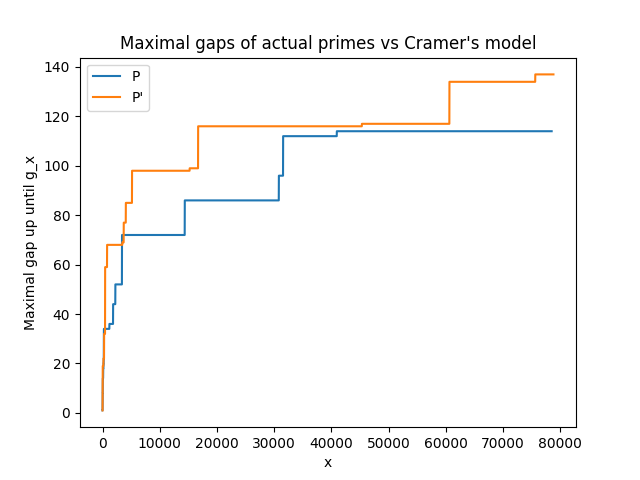
\includegraphics[scale=0.5]{graph.png}
% \inputpython{../models/original_model.py}{6}{37}

\section{Accuracy of the Model}
% You should change this section's name to something relevant to
% your project. This section allows you to reflect or conclude
% the work you have done in your project and discuss future work
% that could be done on the project (e.g. applications you tried
% to make but couldn't find the time).

Under heuristic testing with variations of Cram\'er's model, we should be able to support strong statements such as Bertrand's postulate and Legendre's conjecture. However, comparing with the actual primes, it should be clear that Cram\'er's model is inaccurate. Further work would involve the creation and tuning of other random models, to more closely emulate prime distributions.


\begin{thebibliography}{00}
\bibitem{b1} Terence Tao's Blog
% http://terrytao.wordpress.com/2015/01/04/254a-supplement-4-probabilistic-models-and-heuristics-for-the-primes-optional/#more-7956
\bibitem{b2} Wikipedia Article on Prime Gaps
% https://en.wikipedia.org/wiki/Prime_gap
\end{thebibliography}
\vspace{12pt}

\end{document}
